\documentclass[tikz,border=0pt]{standalone}
\usepackage[utf8]{inputenc}
\usepackage{xcolor}

\newcommand{\cardwidth}{250pt}
\newcommand{\cardheight}{350pt}

\definecolor{cardbg}{HTML}{FFF9C0}
\definecolor{codebg}{HTML}{1A1612}
\definecolor{titlecolor}{HTML}{2D2A24}
\definecolor{bodycolor}{HTML}{4A4540}
\definecolor{categorycolor}{HTML}{888888}
\definecolor{klparen}{HTML}{888888}
\definecolor{klfunction}{HTML}{FF6B6B}
\definecolor{klnumber}{HTML}{4ECDC4}
\definecolor{klvar}{HTML}{95E1D3}
\definecolor{gridcolor}{HTML}{DDDDDD}
\definecolor{boxcolor}{HTML}{FF6B6B}

\begin{document}
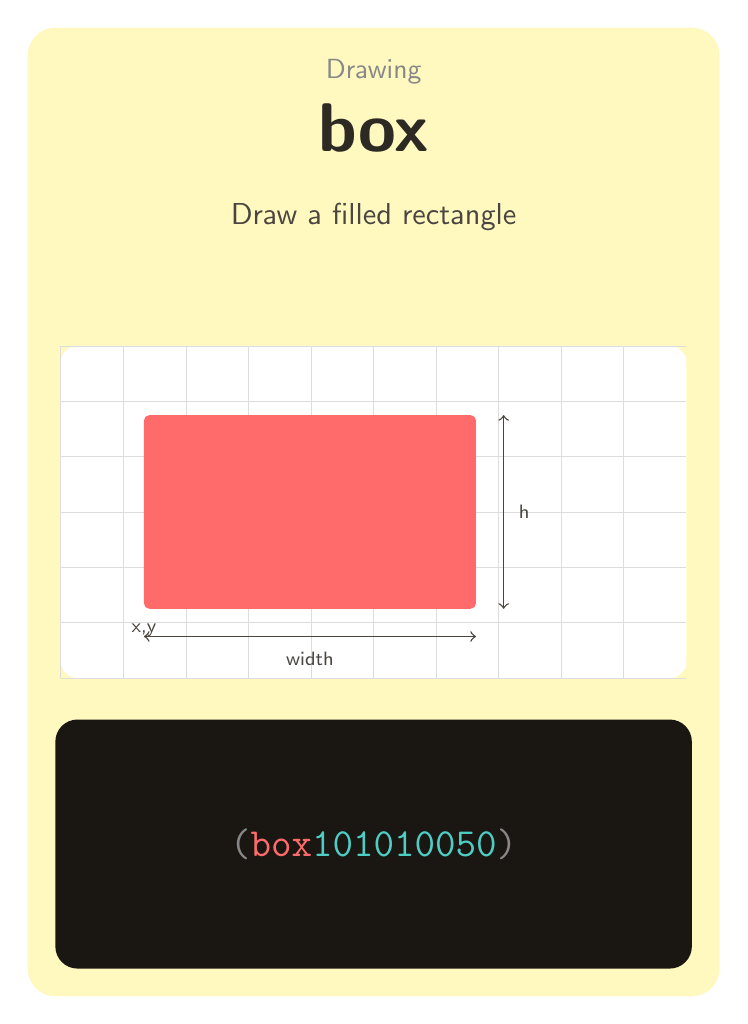
\begin{tikzpicture}
  \fill[cardbg, rounded corners=10pt] (0,0) rectangle (\cardwidth, \cardheight);
  
  \node[anchor=north, font=\sffamily\fontsize{10}{12}\selectfont\color{categorycolor}] 
    at (0.5*\cardwidth, \cardheight-8pt) {Drawing};
  
  \node[anchor=north, font=\sffamily\bfseries\fontsize{28}{32}\selectfont\color{titlecolor}] 
    at (0.5*\cardwidth, \cardheight-24pt) {box};
  
  \node[anchor=north, text width=\cardwidth-24pt, font=\sffamily\fontsize{11}{14}\selectfont\color{bodycolor}, align=center] 
    at (0.5*\cardwidth, \cardheight-60pt) {Draw a filled rectangle};
  
  % === VISUAL DIAGRAM ===
  \begin{scope}[shift={(12pt, 115pt)}]
    \def\diagramwidth{226pt}
    \def\diagramheight{120pt}
    
    \fill[white, rounded corners=6pt] (0,0) rectangle (\diagramwidth, \diagramheight);
    
    \foreach \x in {0,22.6,...,226} {
      \draw[gridcolor, line width=0.3pt] (\x pt, 0) -- (\x pt, \diagramheight);
    }
    \foreach \y in {0,20,...,120} {
      \draw[gridcolor, line width=0.3pt] (0, \y pt) -- (\diagramwidth, \y pt);
    }
    
    % The box itself
    \fill[boxcolor, rounded corners=2pt] (30pt, 25pt) rectangle (150pt, 95pt);
    
    % Dimension labels
    \node[anchor=north, font=\sffamily\fontsize{7}{9}\selectfont\color{bodycolor}] 
      at (30pt, 23pt) {x,y};
    \draw[bodycolor, line width=0.5pt, <->] (30pt, 15pt) -- (150pt, 15pt);
    \node[anchor=north, font=\sffamily\fontsize{7}{9}\selectfont\color{bodycolor}] 
      at (90pt, 13pt) {width};
    \draw[bodycolor, line width=0.5pt, <->] (160pt, 25pt) -- (160pt, 95pt);
    \node[anchor=west, font=\sffamily\fontsize{7}{9}\selectfont\color{bodycolor}] 
      at (162pt, 60pt) {h};
  \end{scope}
  
  % === CODE BLOCK ===
  \fill[codebg, rounded corners=8pt] (10pt, 10pt) rectangle (\cardwidth-10pt, 100pt);
  
  \node[anchor=center] at (0.5*\cardwidth, 55pt) {
    {\fontsize{14}{18}\selectfont\ttfamily
      \textcolor{klparen}{(}%
      \textcolor{klfunction}{box}%
      \textcolor{white}{ }%
      \textcolor{klnumber}{10}%
      \textcolor{white}{ }%
      \textcolor{klnumber}{10}%
      \textcolor{white}{ }%
      \textcolor{klnumber}{100}%
      \textcolor{white}{ }%
      \textcolor{klnumber}{50}%
      \textcolor{klparen}{)}%
    }
  };
\end{tikzpicture}
\end{document}
